\begin{task}
    Рассмотрим задачу

    $$
    \int_{-T_{0}}^{T_{0}} x \sqrt{\dot{x}^{2}+1} d t \rightarrow \min , x\left(T_{0}\right)=x\left(-T_{0}\right)=\xi .
    $$
    
    1) Выписать уравнение Якоби, подобрать одно из его решений, затем найти общее решение.
    
    2) Пусть допустимых экстремалей две. Доказать, что одна из них является точкой сильного минимума, а вторая не является точкой слабого минимума.


    \textbf{Peшение.} 
    У этой задачи мы уже нашли экстремали: $\hat{x}(t)=\frac{1}{c} \mathrm{ch} c t$, где $c>0$ находится из условия с $c T_{0}=c \xi$. Напомним, что существует $\xi_{*}>0$ такое, что при $\xi<\xi_{*}$ решений нет, при $\xi=\xi_{*}$ есть ровно одно решение, при $\xi>\xi_{*}$ есть ровно два решения. При этом в случае $\xi=\xi_{*}$ число $c=c_{*}$ удовлетворяет равенству
    
    $$
    \operatorname{ch} c_{*} T_{0}-c_{*} T_{0} \cdot \operatorname{sh} c_{*} T_{0}=0
    $$
    
    В случае $\xi>\xi_{*}$ выполнено $\operatorname{ch} c_{*} T_{0}<\xi T_{0}$, поэтому одно из решений уравнения $\operatorname{ch} c T_{0}=c \xi$ будет больше $c_{*}$, а второе меньше.
    
    Выпишем уравнение Якоби.
    
    Имеем: $\dot{\hat{x}}(t)=\operatorname{sh} c t, \sqrt{1+\dot{\hat{x}}^{2}(t)}=\operatorname{ch} c t$. Отсюда
    
    $$
    \hat{L}_{\dot{x} \dot{x}}(t)=\frac{1}{c} \cdot \frac{1}{\operatorname{ch}^{2} c t}, \quad \hat{L}_{x \dot{x}}(t)=\frac{\operatorname{sh} c t}{\operatorname{ch} c t}, \quad \hat{L}_{x x}(t)=0 .
    $$
    
    Значит, уравнение Якоби имеет вид
    
    $$
    -\frac{d}{d t}\left(\frac{1}{c} \cdot \frac{1}{\operatorname{ch}^{2} c t} \dot{h}+\frac{\operatorname{sh} c t}{\operatorname{ch} c t} h\right)+\frac{\operatorname{sh} c t}{\operatorname{ch} c t} \dot{h}=0
    $$
    
    После преобразований получаем
    
    $$
    \ddot{h}-2 c \frac{\operatorname{sh} c t}{\operatorname{ch} c t} \dot{h}+c^{2} h=0 \text {. }
    $$
    
    Одно из решений угадывается: $h_{0}(t)=\mathrm{sh} c t$.
    
    Общее решение найдем через определитель Вронского. Напомним, что если $h, w$ - два решения уравнения, то определитель Вронского - это
    
    $$
    W=W(h, w)=\left|\begin{array}{cc}
    h & w \\
    \dot{h} & \dot{w}
    \end{array}\right|=h \dot{w}-w \dot{h} .
    $$
    
    Тогда $\dot{W}=h \ddot{w}-w \ddot{h}=2 c \frac{\mathrm{sh} c t}{\mathrm{ch} c t} W$ (мы воспользовались тем, что $h$ и $w-$ решения дифференциального уравнения). Решим это дифференциальное уравнение на $W$ :
    
    $$
    \dot{W} \cdot \operatorname{ch} c t-2(\operatorname{ch} c t)^{\prime} W=0
    $$
    поделив на $\mathrm{ch}^{3} c t$, получим ( $\left.W \mathrm{ch}^{-2} c t\right)^{\prime}=0$, откуда $W=a \mathrm{ch}^{2} c t$, где $a \in \mathbb{R}$.
    
    Теперь найдем $h$ через $W\left(h_{0}, h\right)$ :
    
    $$
    \dot{h} \operatorname{sh} c t-h(\operatorname{sh} c t)^{\prime}=a \operatorname{ch}^{2} c t
    $$
    
    или
    
    $$
    (h / \operatorname{sh} c t)^{\prime}=a \frac{\operatorname{ch}^{2} c t}{\operatorname{sh}^{2} c t}
    $$
    
    Если $h=z \operatorname{sh} c t$, то $\dot{z}=a \frac{\mathrm{ch}^{2} c t}{\mathrm{sh}^{2} c t}$. Заметим, что $(\operatorname{ch} s / \operatorname{sh} s)^{\prime}=1-(\operatorname{ch} s / \operatorname{sh} s)^{2}$. Отсюда $z=$ $\frac{a}{c}\left(c t-\frac{\mathrm{ch} c t}{\mathrm{sh} c t}\right)+b$, или $h=\frac{a}{c}(c t \mathrm{sh} c t-\mathrm{ch} c t)+b \operatorname{sh} c t$.
    
    Итак, общее решение уравнения Якоби является линейной комбинацией
    
    $$
    h_{0}(t)=\operatorname{sh} c t, \quad h_{1}=\operatorname{ch} c t-c t \operatorname{sh} c t \text {. }
    $$
    
    Функция $h_{0}$ нечетная и строго возрастающая, функция $h_{1}$ четная, $h_{1}(0)>0, h_{1}$ строго возрастает при $t \leq 0$ и строго убывает при $t \geq 0$.
    
    Напомним, что для одного из решений уравнения $\operatorname{ch} c T_{0}=c \xi$ выполнено $c_{1}<c_{*}$, а для другого выполнено $c_{2}>c_{*}$. Значит, при $c=c_{1}$ функция $h_{1}$ будет строго положительной на $\left[-T_{0}, T_{0}\right]$, а при $c=c_{2}$ выполнено $h_{1}\left(-T_{0}\right)<0$.
    
    Пусть $c=c_{1}$. Докажем, что любая нетривиальная линейная комбинация $h_{0}$ и $h_{1}$ имеет не более одного нуля на $\left[-T_{0}, T_{0}\right]$. Для $\alpha h_{0}$ и $\alpha h_{1}$ это понятно. Учитывая четность и нечетность, получаем: достаточно доказать, что при $\alpha>0$ уравнение $h_{1}=\alpha h_{0}$ имеет не более одного корня на $\left[-T_{0}, T_{0}\right]$. В самом деле, $h_{1}(t)>0, h_{0}(t) \leq 0$ при $t \in\left[-T_{0}, 0\right]$. На отрезке $\left[0, T_{0}\right]$ функция $h_{0}$ строго возрастает, а $h_{1}$ строго убывает. Значит, количество корней не более одного.
    
    \begin{figure}[h!]
        \centering
        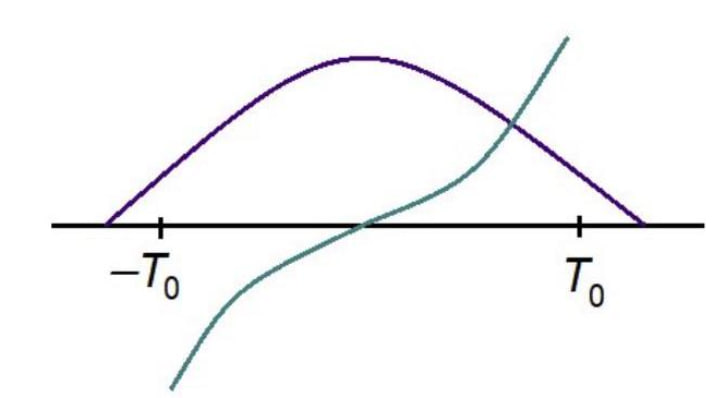
\includegraphics[width=0.99\linewidth]{tasks/task28/pic2.jpg}
    \end{figure}
    
    Таким образом, при $c=c_{1}$ выполнено усиленное условие Якоби.
    
    Пусть $c=c_{2}$. Покажем, что условие Якоби не выполнено. Пусть $h=h_{1}-\alpha h_{0}, h\left(-T_{0}\right)=0$. Тогда $\alpha>0$. Значит, $h(0)>0, h\left(T_{0}\right)<0$. По теореме о промежуточных значениях, $h(\tau)=0$ для некоторого $\tau \in\left(0, T_{0}\right)$.
    
    \begin{figure}[h!]
        \centering
        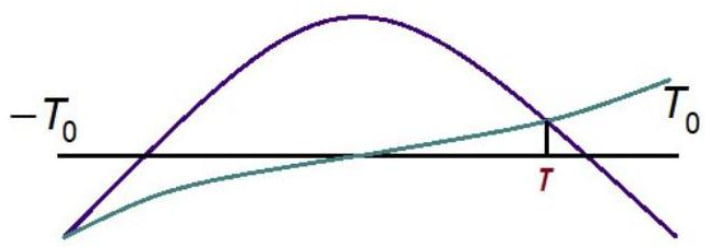
\includegraphics[width=0.99\linewidth]{tasks/task28/pic3.jpg}
    \end{figure}
    
        
    
    Осталось заметить, что при $x>0$ будет выполнено $L_{\dot{x} \dot{x}}=\frac{x}{\left(1+\dot{x}^{2}\right)^{3 / 2}}>0$. Значит, выполнено усиленное условие Лежандра и усиленное условие Вейерштрасса. Поэтому в первом случае будет сильный минимум, а во втором не будет слабого минимума.

\end{task}